\documentclass{tufte-handout}

\usepackage{fancyvrb}
\fvset{fontsize=\normalsize}

\usepackage{hyperref}
\hypersetup{colorlinks=true}

\usepackage{graphicx}

% Hide page numbers in ToC
\let\Contentsline\contentsline
\renewcommand\contentsline[3]{\Contentsline{#1}{#2}{}}

\title{Systems Management with Matahari}
\author{\href{mailto:zbitter@redhat.com}{Zane Bitter}}
\date{5 February 2012}

\begin{document}
\maketitle

\marginnote{\tableofcontents \vspace{2em}}

\begin{abstract}
An introduction to the \href{http://matahariproject.org}{Matahari Project} for developers, system administrators and the Open Source community.
\end{abstract}

\section{Introducing Matahari}

Matahari is a framework for remote systems management. Unlike traditional methods of remote management (e.g. SSH), it is designed for programmatic as well as manual access, and to work with large numbers of machines as might be found in a modern ``cloud'' installation.

\begin{figure*}[b!]
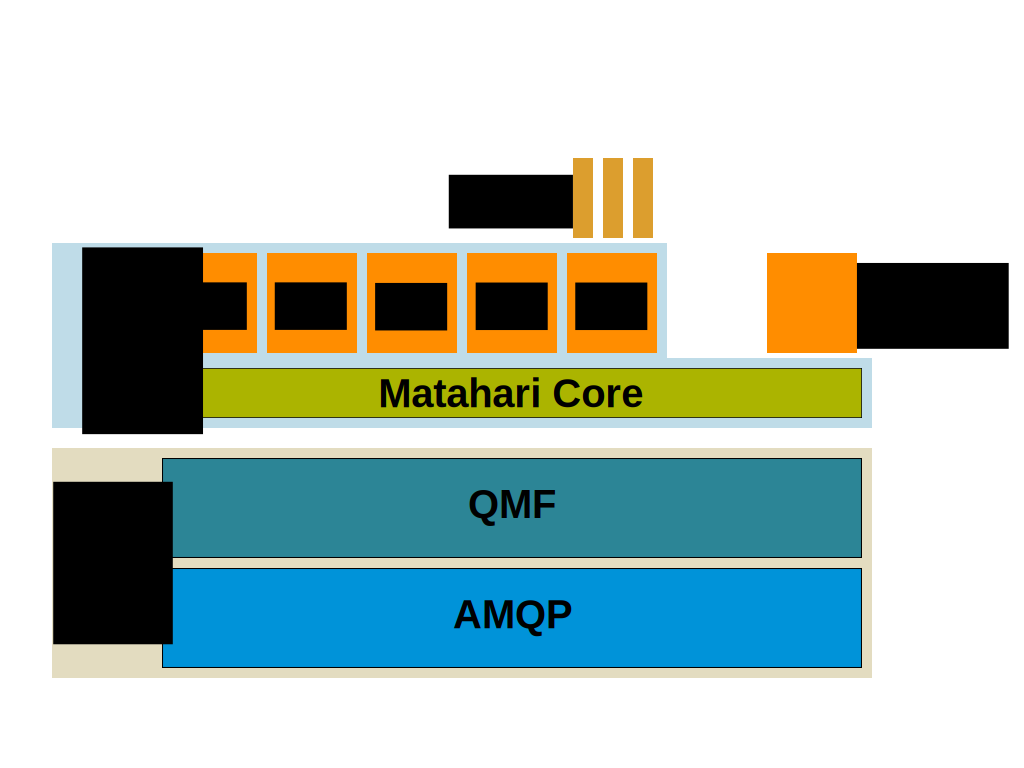
\includegraphics[trim=3em 9em 0 14em,width=\textwidth]{arch.pdf}
\caption{High-level architecture of Matahari and related projects.}
\label{fig:arch}
\end{figure*}

Matahari messages use the Advanced Message Queueing Protocol (AMQP) as a transport. This allows for a very flexible and scalable messaging architecture, with the ability to efficiently manage a large network of machines.
Matahari exposes remote APIs as objects with properties, methods and events which are exported by the Qpid Management Framework. QMF provides an object modelling layer with remote method invocation and introspection. It is developed as part of and runs atop Apache Qpid, a popular implementation of AMQP.\footnote{In the future we will investigate breaking this dependency, hopefully to the point where QMF could run on top of other AMQP implementations.}

In addition to the bus architecture of AMQP, QMF supports asynchronous method calls and publish-subscribe semantics for events. These features also help make it very suitable for large-scale deployments.

\section{Matahari Agents}

Matahari ships with a number of agents that export useful APIs. At present, Matahari includes Host (generic hardware information), Network (network interfaces), Sysconfig (Puppet and Augeas configuration), Service (system services) and RPC agents.
Many of these agents support Windows as well as Linux hosts, so they can be used on Windows-based virtualised guests.

More agents are planned, in particular for package management.
However, the Matahari project itself is not intended to be the source of all system APIs. Rather, Matahari seeks to provide access to its infrastructure so that developers from other projects can create third-party agents to expose their own APIs.

\subsection{RPC Agent}

The RPC agent allows developers or system administrators to add their own custom functionality to Matahari without the overhead of developing a new agent in C++. The combination of Matahari and RPC plugins offers functionality similar to MCollective.

The RPC agent exports any Python module stored in the directory \Verb|/usr/lib/matahari/plugins| as a plugin object in QMF. Every public, callable attribute of the module is exported as a method of the plugin object. Parameters are passed and results returned in \smallcaps{JSON} format.

\begin{figure}[hb]
\begin{Verbatim}
import subprocess

def num_calls():
    cl_args = ["asterisk", "-rx", "core show channels count"]
    return subprocess.check_output(cl_args)
\end{Verbatim}
\caption{An example RPC plugin for getting the number of calls from an Asterisk server. The \texttt{num\_calls} function will be exported as a method of a QMF class named after the module. See Figure \ref{fig:shell} for an example use.}
\label{fig:rpc}
\end{figure}

Support for a Ruby backend would be a desirable future addition.

\section{Core Libraries}

The core of Matahari (see Figure~\ref{fig:arch}) comprises code that creates the skeleton structure of a Matahari agent and links it with QMF. Both agents that ship with Matahari and external agents such as libvirt-qmf share this same core.

Every Matahari agent shares common configuration files, command line options, environment variables and the like, to ensure that the entire suite of agents running on a system need only be configured once.

\begin{figure}[h]
\begin{Verbatim}
<schema package="org.matahariproject.testagent">
    <class name="TestClass">
        <property name="hostname" type="sstr" access="RO" desc="Hostname" index="y" />

        <method name="sum" desc="Sum of two numbers">
            <arg name="x" dir="I" type="int32" />
            <arg name="y" dir="I" type="int32" />
            <arg name="result" dir="O" type="int32" />
        </method>
    </class>
</schema>
\end{Verbatim}
\caption{The example agent schema.}
\label{fig:schema}
\end{figure}

\begin{figure}[hbt]
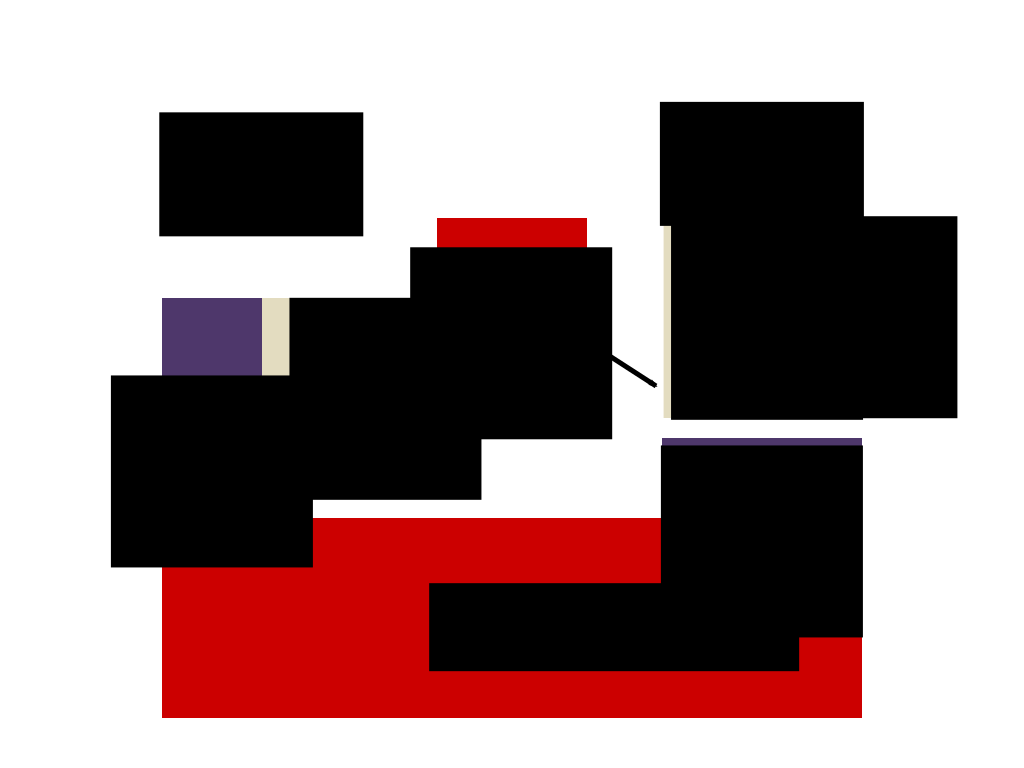
\includegraphics[trim=0 9em 0 12em,width=\textwidth]{agent-arch.pdf}
\caption{Components of a Matahari agent.}
\label{fig:agent-arch}
\end{figure}

The API of an agent is described by a \href{https://cwiki.apache.org/qpid/qpid-management-framework.html#QpidManagementFramework-Schema}{QMF Schema}, which defines events and the classes of objects and their properties and methods. As shown in Figure~\ref{fig:agent-arch}, Matahari includes tools to transform the XML schema into code to create the necessary classes in QMF.
It also includes tools to (optionally) generate the skeleton of a D-Bus API from the same schema, so that the same API can be accessed locally via D-Bus on Linux systems.\footnote{The included Host, Network, Sysconfig and Service APIs supply D-Bus as well as QMF agents.}

The underlying functionality of the API is usually encapsulated in a shared library. It is envisioned that for most third-party agents this will be an existing C API. In that case, the developer need only write the glue code for each of the QMF and D-Bus agents to link the underlying API to the generated schema.

Developers of third-party agents should begin by forking the \href{https://github.com/matahari/matahari-agent-example}{example agent repository} on GitHub and adapting it to their needs.\footnote{For more information, read the \href{https://github.com/downloads/zaneb/presentations/matahari-for-developers-7db27de.pdf}{Introduction to Matahari for Developers}.}

\section{Clients}

\begin{marginfigure}
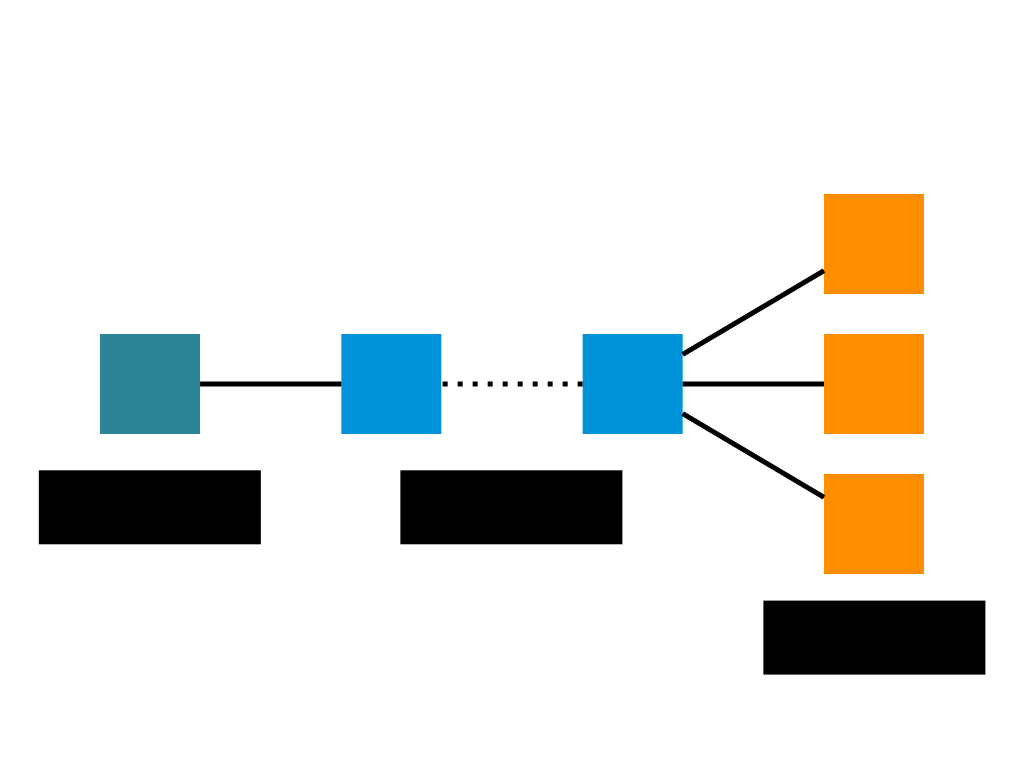
\includegraphics[trim=0 8em 0 8em,width=\textwidth]{qmf-terminology.pdf}
\caption{Anatomy of a QMF system}
\label{fig:qmf-terminology}
\end{marginfigure}

In QMF terminology, client applications are known as ``consoles''. Consoles connect to agents through one or more message brokers. Broker Federation can be used to set up a network of interconnected brokers.

\begin{figure}[b]
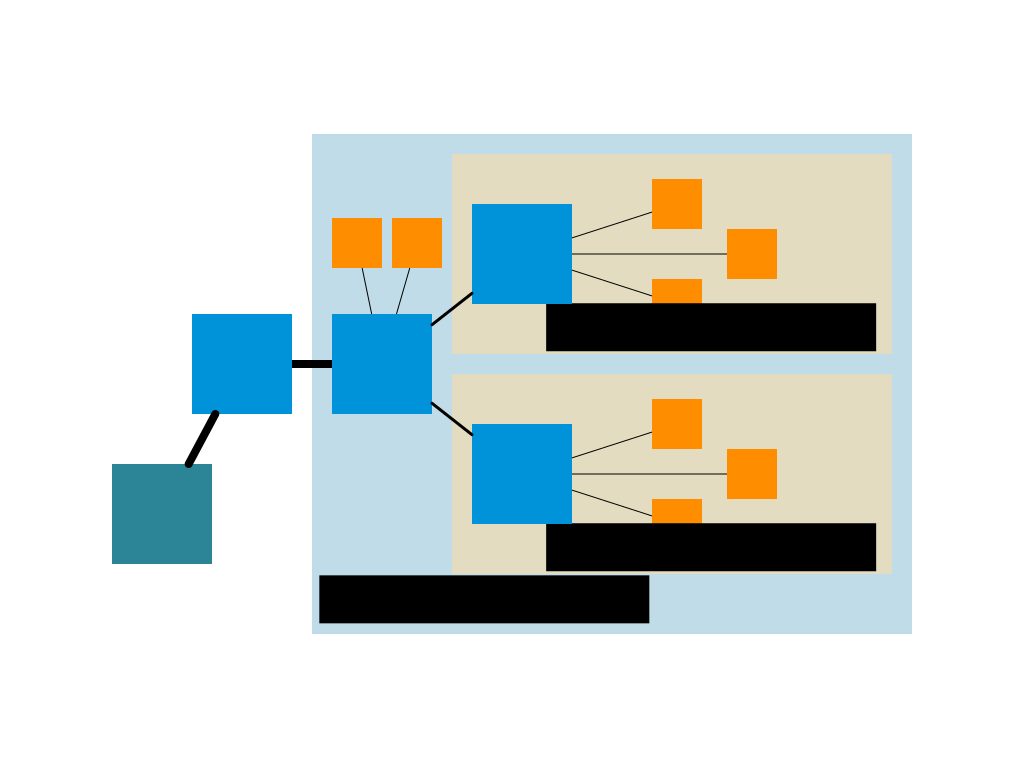
\includegraphics[trim=0 12em 0 12em,width=\textwidth]{vhost-topology.pdf}
\caption{A typical Matahari QMF Bus topology in a virtualised environment.}
\label{fig:vhost-topology}
\end{figure}

In a typical Matahari setup agents connect to a local broker running on the same host. The local broker may federate with an external broker to allow centralised management of a group of machines.
In a virtualised environment, illustrated in Figure~\ref{fig:vhost-topology}, local brokers on the guests can federate with a broker running on the host through a \smallcaps{QEMU} vios-proxy tunnel.
 
Matahari installs its own broker, which is simply a thin wrapper around the Apache Qpid broker to read Matahari-specific configuration. In this way, Matahari can be kept completely separate from any other use of AMQP in the network.\footnote{By default, the Matahari broker uses its own TCP port, 49000, to listen for incoming connections.}

There are QMF console libraries available in C++, Python and Ruby.
In addition, there is a Matahari API in Python under active development.\footnote{A preview is available now in the Matahari Git repository.} This API simplifies common systems-management tasks that are specific to Matahari rather than generic to QMF, such as selecting agents by host. It also provides an easy mechanism for using asynchronous QMF operations to deal with many agents in parallel.

\subsection{Applications}

Matahari is already in use by the \href{http://pacemaker-cloud.org/}{Pacemaker Cloud} project to remotely monitor the state of system services using push notifications. The Cloud Policy Engine acts as a Matahari console to control and monitor services.

\subsection{Matahari Shell}

The Matahari Shell (\texttt{mhsh}) is a wrapper around the Matahari Python API.\footnote{Like the API, the shell is still under active development and is subject to change, but available to preview now.} It allows the user to interact with remote agents using a command-line interface,\footnote{The interface should feel at least somewhat familiar to anyone who has used Cisco's IOS, or any of the many similar command lines.} or to drive them from a script.

The strategy for using the shell is to select a subset of the available objects and perform operations on the whole group.
The user selects an object class and, optionally, a list of hosts and property values on which to filter.
The shell inherits from the API the ability to dispatch method calls to every selected object in parallel.

\begin{figure*}[hb]
\begin{Verbatim}
$ mhsh
mhsh> list hosts
ast1
ast2
mhsh> select class package org.matahariproject.rpc.plugin asterisk
mhsh [org.matahariproject.rpc.plugin:calls]> call num_calls
OK (0) - {u'result': '"0 active channels\\n0 active calls\\n0 calls processed\\n"'}
OK (0) - {u'result': '"0 active channels\\n0 active calls\\n0 calls processed\\n"'}
mhsh [org.matahariproject.rpc.plugin:calls]> select class Host
mhsh [org.matahariproject:Host]> select host ast1
mhsh (host)[org.matahariproject:Host]> get load
{u'1': 0.0, u'5': 0.01, u'15': 0.05}
mhsh (host)[org.matahariproject:Host]> quit
$
\end{Verbatim}
\caption{An example shell session. First we call the \texttt{num\_calls} method from the RPC plugin of Figure \ref{fig:rpc} on all hosts where it is present. Then we select a single host and get its load average from the Host agent.}
\label{fig:shell}
\end{figure*}


\section{More Information}

Here is a list of other places you can go to get more information and participate in the project:

\begin{itemize}
\item The project home page is \url{http://matahariproject.org/}.
\item You can find the code on \href{https://github.com/matahari/matahari}{GitHub}.
\item Patches and project-related discussions are posted to the \href{https://fedorahosted.org/mailman/listinfo/matahari}{Matahari mailing list}.
\item Developers and users hang out in the \texttt{\#matahari} IRC channel on \href{http://www.oftc.net/}{OFTC}.
\end{itemize}

\end{document}
